\documentclass[11pt]{article}
\usepackage[margin=2.2cm]{geometry}
\usepackage{booktabs}
\usepackage{siunitx}
\usepackage{array}
\usepackage{caption}
\usepackage{pgfplots}
\pgfplotsset{compat=1.18}
\sisetup{group-separator={,},group-minimum-digits=4}

\newcommand{\cfg}[1]{\texttt{#1}}

\title{AskMH RAG Agent: LLM Comparison\\\large Gemini 2.5 Flash (thinking off vs.\ dynamic) and Qwen3-8B}
\date{Runs recorded 16 October 2026}
\author{}

\begin{document}
\maketitle

\section{Setup}

\begin{table}[h]
\centering
\caption{Configurations under test. All share the same retrieval: \cfg{bge-base-en-v1.5} embeddings, Chroma index of 1{,}526 chunks, top-$k=5$ articles.}
\begin{tabular}{@{}llll@{}}
\toprule
 & \cfg{gemini-off} & \cfg{gemini-dynamic} & \cfg{qwen} \\
\midrule
Model       & \cfg{gemini-2.5-flash} & \cfg{gemini-2.5-flash} & \cfg{qwen3:8b} (Ollama) \\
Thinking    & budget $=0$            & budget $=-1$ (dynamic) & reasoning off \\
Temperature & 0                      & 0                      & 0 \\
Seed        & n/a                    & n/a                    & 42 \\
Hardware    & Google API             & Google API             & RTX 4060 Laptop, 8\,GB \\
\bottomrule
\end{tabular}
\end{table}

Dataset: 50 LLM-paraphrased FAQ questions over 42 topics, one labelled source article each.
Two runs per configuration (300 agent turns). \emph{Accuracy} (\cfg{cited\_expected}) means the
outcome is \emph{answered} and the labelled article is among the cited sources.

\section{Outcomes and accuracy}

\begin{table}[h]
\centering
\caption{Outcomes per run ($n=50$). Retrieval hit = labelled article in the top 5; run 1 of Gemini did not record retrieval.}
\label{tab:outcomes}
\begin{tabular}{@{}lccccccc@{}}
\toprule
Run & Answered & \textbf{Accuracy} & Clarify & Declined & Handoff & Error & Retrieval hit \\
\midrule
\cfg{gemini-off} r1     & 36 & \textbf{36} & 7  & 6  & 1 & 0 & n/a \\
\cfg{gemini-off} r2     & 36 & \textbf{36} & 7  & 6  & 1 & 0 & 43 \\
\cfg{gemini-dynamic} r1 & 38 & \textbf{36} & 8  & 3  & 1 & 0 & n/a \\
\cfg{gemini-dynamic} r2 & 39 & \textbf{37} & 7  & 3  & 1 & 0 & 44 \\
\cfg{qwen} r1           & 22 & \textbf{22} & 16 & 12 & 0 & 0 & 45 \\
\cfg{qwen} r2           & 22 & \textbf{22} & 16 & 12 & 0 & 0 & 45 \\
\bottomrule
\end{tabular}
\end{table}

\begin{figure}[h]
\centering
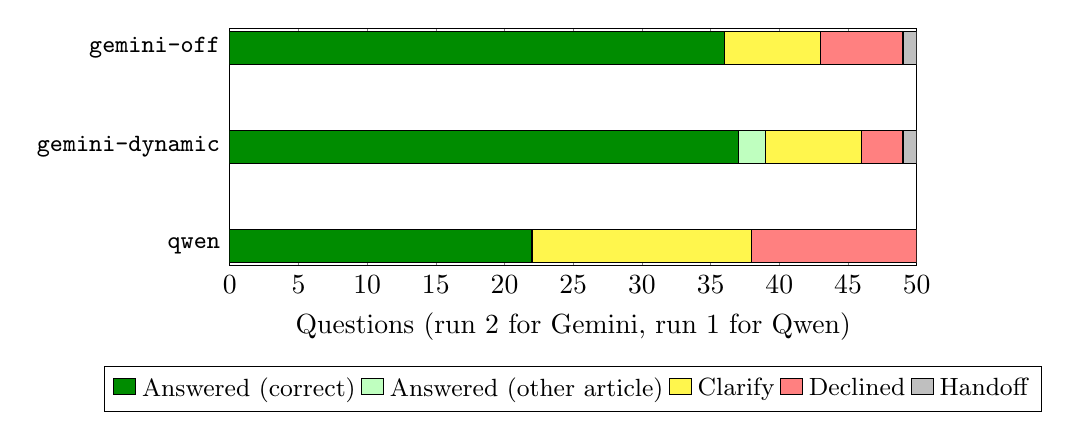
\begin{tikzpicture}
\begin{axis}[
    xbar stacked,
    width=0.85\textwidth,
    height=4.6cm,
    bar width=12pt,
    xmin=0, xmax=50,
    xlabel={Questions (run 2 for Gemini, run 1 for Qwen)},
    symbolic y coords={qwen,gemini-dynamic,gemini-off},
    ytick=data,
    yticklabel style={font=\ttfamily\small},
    legend style={at={(0.5,-0.42)},anchor=north,legend columns=-1,font=\small},
    reverse legend=false,
]
\addplot[fill=green!55!black] coordinates {(36,gemini-off) (37,gemini-dynamic) (22,qwen)};
\addplot[fill=green!25]       coordinates {(0,gemini-off) (2,gemini-dynamic) (0,qwen)};
\addplot[fill=yellow!70]      coordinates {(7,gemini-off) (7,gemini-dynamic) (16,qwen)};
\addplot[fill=red!50]         coordinates {(6,gemini-off) (3,gemini-dynamic) (12,qwen)};
\addplot[fill=gray!50]        coordinates {(1,gemini-off) (1,gemini-dynamic) (0,qwen)};
\legend{Answered (correct), Answered (other article), Clarify, Declined, Handoff}
\end{axis}
\end{tikzpicture}
\caption{Outcome distribution per configuration.}
\label{fig:outcomes}
\end{figure}

\section{Latency}

\begin{table}[h]
\centering
\caption{Whole-turn wall time in seconds, first question excluded ($n=49$). The maximum for every Gemini run is q004 (degenerate router output).}
\label{tab:latency}
\begin{tabular}{@{}lS[table-format=2.2]S[table-format=1.2]S[table-format=1.2]S[table-format=3.2]@{}}
\toprule
Run & {Mean} & {Median} & {p90} & {Max} \\
\midrule
\cfg{gemini-off} r1     & 6.33  & 3.82 & 4.39 & 136.22 \\
\cfg{gemini-off} r2     & 5.31  & 3.91 & 4.22 & 88.66 \\
\cfg{gemini-dynamic} r1 & 11.91 & 6.67 & 9.10 & 254.93 \\
\cfg{gemini-dynamic} r2 & 14.75 & 6.56 & 9.14 & 259.34 \\
\cfg{qwen} r1           & 2.70  & 2.42 & 4.23 & 6.52 \\
\cfg{qwen} r2           & 3.42  & 3.21 & 4.75 & 8.84 \\
\bottomrule
\end{tabular}
\end{table}

Excluding q004 as well ($n=48$): \cfg{gemini-off} mean 3.57\,s (max 4.32\,s),
\cfg{gemini-dynamic} mean 9.65\,s (max 98.3\,s), \cfg{qwen} mean 2.72\,s (max 6.52\,s).

\begin{table}[h]
\centering
\caption{Median duration of each graph step in seconds (run 2 for Gemini, run 1 for Qwen).}
\label{tab:steps}
\begin{tabular}{@{}lccc@{}}
\toprule
Step & \cfg{gemini-off} & \cfg{gemini-dynamic} & \cfg{qwen} \\
\midrule
Router   & 1.32 & 1.55          & 0.80 \\
Retrieve & 0.05 & 0.05          & 0.01 \\
Grade    & 1.33 & \textbf{2.63} & 0.87 \\
Generate & 1.30 & \textbf{2.09} & 1.44 \\
\bottomrule
\end{tabular}
\end{table}

\section{Tokens and cost}

\begin{table}[h]
\centering
\caption{Token totals over 50 questions. Cost at assumed list price: \$0.30 / 1M input, \$2.50 / 1M output (thinking billed as output).}
\label{tab:tokens-all}
\begin{tabular}{@{}lS[table-format=6.0]S[table-format=6.0]S[table-format=5.0]l@{}}
\toprule
Run & {Input} & {Output} & {Thinking} & Cost \\
\midrule
\cfg{gemini-off} r2     & 53309  & 25259  & 0     & \$0.079 \\
\cfg{gemini-dynamic} r2 & 170268 & 107487 & 37940 & \$0.320 \\
\cfg{qwen} r1           & 51525  & 4514   & 0     & local \\
\bottomrule
\end{tabular}
\end{table}

\begin{table}[h]
\centering
\caption{Token totals excluding the q004 outlier ($n=49$).}
\label{tab:tokens-ex}
\begin{tabular}{@{}lS[table-format=5.0]S[table-format=5.0]S[table-format=5.0]S[table-format=3.0]l@{}}
\toprule
Config & {Input} & {Output} & {Thinking} & {Output / q} & Cost / q \\
\midrule
\cfg{gemini-off}     & 52185 & 3719  & 0     & 76  & \textbf{\$0.0005} \\
\cfg{gemini-dynamic} & 54260 & 41568 & 37533 & 848 & \textbf{\$0.0024} \\
\cfg{qwen}           & 50597 & 4442  & 0     & 91  & n/a \\
\bottomrule
\end{tabular}
\end{table}

\section{Stability and divergence}

\begin{table}[h]
\centering
\caption{Run-to-run stability at temperature 0.}
\label{tab:stability}
\begin{tabular}{@{}lcp{8.5cm}@{}}
\toprule
Config & Outcomes changed & Notes \\
\midrule
\cfg{qwen}           & 0/50 & Rewrites and token totals identical \\
\cfg{gemini-off}     & 0/50 & Output tokens differed by 1--9 on 9 questions; q004 length varies \\
\cfg{gemini-dynamic} & 1/50 & q033: clarify $\rightarrow$ answered (correct) \\
\bottomrule
\end{tabular}
\end{table}

\begin{table}[h]
\centering
\caption{Where configurations diverge, attributed to the first pipeline step that disagrees (run 2).}
\label{tab:divergence}
\begin{tabular}{@{}lcccccc@{}}
\toprule
Comparison & Differ & Router & Retrieval & Grader & Generator & Gained / lost \\
\midrule
\cfg{gemini-off} $\rightarrow$ \cfg{gemini-dynamic} & 8  & 3 & 1 & 4  & 0 & $+3$ / $-2$ \\
\cfg{qwen} $\rightarrow$ \cfg{gemini-off}           & 26 & 3 & 2 & 19 & 2 & $+16$ / $-2$ \\
\cfg{qwen} $\rightarrow$ \cfg{gemini-dynamic}       & 24 & 2 & 2 & 18 & 2 & $+16$ / $-1$ \\
\bottomrule
\end{tabular}
\end{table}

\section{Summary}

\begin{table}[h]
\centering
\caption{Headline comparison (run 2 for Gemini, run 1 for Qwen; latency and cost exclude q004).}
\label{tab:summary}
\begin{tabular}{@{}lccc@{}}
\toprule
Metric & \cfg{gemini-off} & \cfg{gemini-dynamic} & \cfg{qwen} \\
\midrule
Accuracy (cited correct article) & \textbf{36/50 (72\%)} & 37/50 (74\%) & 22/50 (44\%) \\
Median latency                   & 3.91\,s & 6.56\,s & \textbf{2.42\,s} \\
Mean latency                     & 3.57\,s & 9.65\,s & \textbf{2.72\,s} \\
Output tokens / question         & \textbf{76} & 848 & 91 \\
Cost / question                  & \$0.0005 & \$0.0024 & \textbf{free (local)} \\
Outcomes changed across runs     & \textbf{0/50} & 1/50 & \textbf{0/50} \\
\bottomrule
\end{tabular}
\end{table}

\noindent\textbf{Decision.} Deploy Gemini 2.5 Flash with thinking off: accuracy equal to dynamic thinking
(within noise), about $1.7\times$ faster at the median and $5\times$ cheaper per question. Gemini resolves
64\% more questions than Qwen3-8B, almost entirely because its grader commits to an answer where Qwen
asks for clarification or declines.

\end{document}
